\subsection{GPU algorithm}

This is a custom approach, aimed at maximising parallelization on GPU.
% This approach aims to leverage the GPU for finding bubbles 

\subsubsection{Algorithm}

The algorithm analyzes each pixel in GPU, to then collect the results with a CPU portion:
\begin{enumerate}
	\itemsep 0em
	\item For each possible radius $r$ between 1 and a parameter \texttt{MAX\_RADIUS}, execute a GPU kernel for each image pixel. The kernel operates the following:
	      \begin{enumerate}
		      \item Using Bresenham's rasterization algorithm, find the list of points that compose the circle of radius $r$ around the pixel of the thread;
		      \item Find the fraction of ``on'' pixels among these;
		      \item Decide if the pixel can be a bubble or not, based on the following conditions:
		            \begin{itemize}
			            \item If within \texttt{MAX\_RADIUS} there is already a bubble, this cannot be another one (to avoid finding the same bubble twice);
			            \item If the pixel has $100\%$ score, and the surrounding pixels have a lower score, then the pixel is considered to be a bubble;
			            \item If this pixel was already marked as bubble in a previous iteration, leave it as it is;
			            \item If none of the previous conditions hold, and $r$ is not \texttt{MAX\_RADIUS}, continue to the next iteration;
			            \item If $r$ is \texttt{MAX\_RADIUS} and the pixel is a local maximum, consider it as a bubble;
			            \item Otherwhise, the pixel is not a bubble.
		            \end{itemize}
	      \end{enumerate}
	\item In CPU, collect all the pixels marked as ``bubble'' into a common list.
\end{enumerate}

\subsubsection{Evaluation}

While useful as a learning tool, this approach yielded poor results: speed was just reaching 15 FPS, and only 43\% of the bubbles were identified, as visible in figure~\ref{fig:locate:gpu}.

\begin{figure}[H]
	\centerline{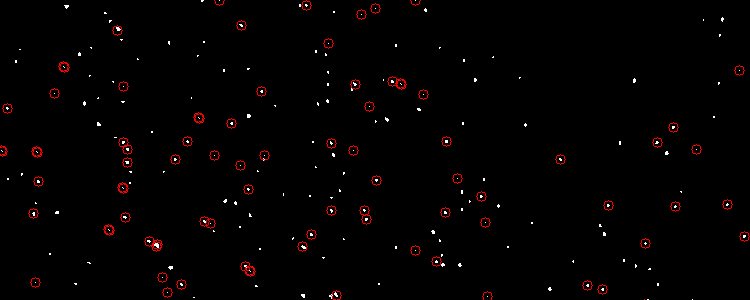
\includegraphics[width=\locateimgsize]{images/locate/my-gpu-algorithm.png}}
	\caption{\centering GPU algorithm's result}
	\label{fig:locate:gpu}
\end{figure}
